\documentclass[11pt, oneside]{article}   	% use "amsart" instead of "article" for AMSLaTeX format
\usepackage{geometry}                		% See geometry.pdf to learn the layout options. There are lots.
\geometry{letterpaper}                   		% ... or a4paper or a5paper or ... 
%\geometry{landscape}                		% Activate for for rotated page geometry
%\usepackage[parfill]{parskip}    		% Activate to begin paragraphs with an empty line rather than an indent
\usepackage{graphicx}				% Use pdf, png, jpg, or eps� with pdflatex; use eps in DVI mode
								% TeX will automatically convert eps --> pdf in pdflatex		
\usepackage{amssymb}
\usepackage{amsmath}
\usepackage{parskip}
\usepackage{color}
\usepackage{hyperref}

\title{Integrate 1/z}
%\author{The Author}
%\section{}
%\subsection*{}
\date{}							% Activate to display a given date or no date

\graphicspath{{/Users/telliott_admin/Dropbox/Tex/png/}}
% \begin{center} 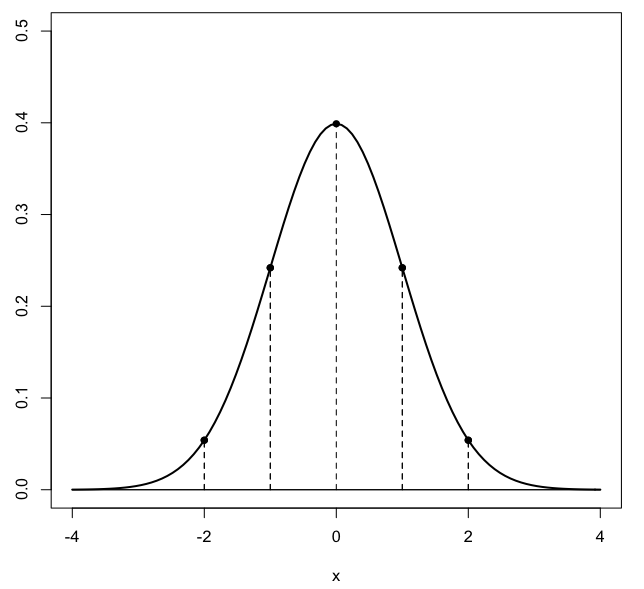
\includegraphics [scale=0.4] {gauss3.png} \end{center}
\begin{document}
\maketitle
\Large

\[ \int_0^{2\pi} \frac{1}{z} \ dz \]

Examining the inverse function, let's first confirm that it is analytic by calculating the partial derivatives.  We have
\[ \frac{1}{z} = \frac{1}{x + iy} \]
One way to simplify is to multiply on top and bottom by $z*$:
\[ = \frac{1}{x + iy} \ \frac{x-iy}{x- iy} \]
\[ = \frac{x - iy}{x^2 + y^2} \]
Thus
\[ u = \frac{x}{x^2 + y^2} \]
\[ u_x = \frac{(x^2 + y^2) - 2x^2}{(x^2 + y^2)^2} = \frac{y^2 - x^2}{(x^2 + y^2)^2} \]
\[ u_y = \frac{-2xy}{(x^2 + y^2)^2} \]
And
\[ v =  \frac{-y}{x^2 + y^2} \]
\[ v_y = - \frac{(x^2 + y^2) - 2y^2}{(x^2 + y^2)^2} = \frac{y^2 - x^2}{(x^2 + y^2)^2} \]
\[ v_x = \frac{2xy}{(x^2 + y^2)^2} \]
CRE are satisfied and the inverse of $z$ is indeed analytic.

If we are on the unit circle, then 
\[ z = e^{i\theta} \]
\[ dz = ie^{i\theta} d \theta \]
\[ \int \frac{dz}{z} = \int e^{-i\theta} \ i  e^{i \theta} \ d \theta = 2 \pi i \]

If we're centered on the origin but we don't have a unit circle, there will be an $R$ in both the numerator and the denominator, which cancel.  The result is thus independent of the radius of the circle.

In general
\[ \oint_C \frac{dz}{(z - z_0)^n} = 
\begin{cases}
0, & n \ne 1 \\
2 \pi i, & n = 1 
\end {cases}
\]

We can also integrate the inverse function in terms of $x$ and $y$:
\[ \oint \frac{1}{z} \ dz = \oint \frac{dx + i dy}{x + iy} \]
\[ = \oint \frac{1}{x^2+y^2} \ [ \  x \ dx - y \ dy + i x \ dy + i y \ dx \ ] \]
Suppose we go on a circle of radius $R$ centered on the origin and parametrize in terms of $\theta$.  We obtain:
\[ x = R \cos \theta \]
\[ y = R \sin \theta \]
\[ x^2 + y^2 = R^2 \]
\[ dx = - R \sin \theta \ d \theta \]
\[ dy = R \cos \theta \ d \theta \]
We have for the integral
\[ \oint \frac{1}{x^2+y^2} \ [ \  x \ dx - y \ dy + i x \ dy + i y \ dx \ ] \]
\[ = \int \frac{1}{R^2} \ [ \ -R^2 \cos \theta \sin \theta \ d \theta + R^2 \sin \theta \cos \theta \ d \theta + i R^2 \cos^2 \theta \ d \theta + i R^2 \sin^2 \theta \ d \theta \ ] \]
\[ = \int \frac{1}{R^2} \ [ \ i R^2 \cos^2 \theta \ d \theta + i R^2 \sin^2 \theta \ d \theta \ ] \]
\[ = \int i \cos^2 \theta \ d \theta + i \sin^2 \theta \ d \theta \]
\[ = \int i \ d \theta = 2 \pi i \]

Note that if we integrate the same function around a unit square, we run into problems.  First let's  do $[0,0 \times 1,1]$.  We have
\[ \int u \ dx - \int v \ dy + i \ [ \ \int v \ dx + \int u \ dy \ ]  \]
Along $C1$, $y = 0$ and $dy = 0$ so:
\[ \int \frac{x}{x^2 + y^2} \ dx + i \ [ \ \int \frac{-y}{x^2 + y^2} \ dx \]
\[ = \int_0^1 \frac{1}{x} \ dx = \ln x \ \bigg |_0^1 \]
Since $\ln 0$ is not defined, we can't do this.

Logarithms are tricky, no doubt.  If the complex logarithm $Log z$ is defined and differentiable along the curve (say the semicircle from $-i$ to $i$), we can do this:
\[ I = \int_{-i}^i \frac{1}{z} \ dz = Log z \ \bigg |_{-i}^i  \]
Recall that $z = re^{i\theta}$ with $r=1$ so this is
\[ = (\ln 1 + i \ \frac{\pi}{2} ) - (\ln 1 + i \frac{-\pi}{2} ) = 2i \ \frac{\pi}{2} = \pi i \]
For any value of $r$ (except $r=0$), we get the same answer, since $\ln r - \ln r = 0$.

\subsection*{example}
We can extend this to 
\[ \oint \frac{1}{z^2} \ dz \]
As before, on the unit circle
\[ z = e^{i\theta} \]
\[ dz = i z \ d \theta \]
so the integral is
\[ \int_0^{2 \pi} \ \frac{i}{z} \ d \theta =  \int_0^{2 \pi} i e^{-i\theta} \ d \theta \]
Now
\[ \int e^{-i\theta} \ d \theta = -i e^{-i\theta} \]
so cancel $i \cdot -i$ and we have just
\[ = e^{-i\theta} \ \bigg |_0^{2 \pi}  \]
Evaluate the first term using Euler's formula:
\[ e^{-2\pi i} = \cos -2 \pi + i \sin -2 \pi \]
\[ = \cos 2 \pi - i \sin 2 \pi = 1 \]
So the whole thing is zero.

In fact, for any negative integer power of $z$
\[ \int z^{-n} \ dz \]
around the unit circle $z=e^{i\theta}$ we have
\[ i \int e^{-i(n-1)\theta} \ d \theta \]
\[ = \frac{1}{n-1} \ e^{-i(n-1)\theta} \ \bigg |_0^{2 \pi}  \]
\[ = \frac{1}{n-1} \ [ \ (\cos 2 (n-1) \pi - i \sin 2 (n-1) \pi ) \ - 1 ]   \]
\[ = \frac{1}{n-1} \ [ \ 1  - 1 ] \ = 0  \]

\end{document}  